% Nome del file: ManualeUtente.tex
% Percorso: \gl{template}
% Autore: Vault-Tech
% Data creazione: 10.05.2016
% E-mail: vaulttech.swe@gmail.comcom
%
% Diario delle modifiche: interno al file.

\documentclass[a4paper, titlepage]{article}

\usepackage[margin=3cm]{geometry}
\usepackage{../../Stile}
\usepackage{../../Comandi}

\setcounter{secnumdepth}{5}
\setcounter{tocdepth}{5}

\def\NOME{Manuale Utente}
\def\VERSIONE{1.0}
\def\DATA{12.05.2016}
\def\REDATTORE{Michela De Bortoli \\ & Filippo Tesser}
\def\VERIFICATORE{Miki Violetto}
\def\RESPONSABILE{Giacomo Beltrame}
\def\USO{Esterno}
\def\DISTRIBUZIONE{\COMMITTENTE \\ & \CARDIN \\ & \PROPONENTE}


\begin{document}
	
	\pagestyle{fancy}	
	\pagenumbering{Roman}
	\rfoot{Pagina \thepage{} di \pageref{lastromanpage}}
	
	\maketitle
	
	\begin{diario}
	\recap{Approvazione del documento}{Michela De Bortoli}{Responsabile}{06.04.2016}{3.0}
	\recap{Correzione errori individuati}{Michela De Bortoli}{Analista}{06.04.2016}{2.10}
	\recap{Verifica dell'intero documento}{Rudy Berton}{Verificatore}{05.04.2016}{2.9}
	\recap{Stesura appendice D}{Giacomo Beltrame}{Analista}{04.04.2016}{2.8}
	\recap{Verifica appendici A e B}{Giacomo Beltrame}{Verificatore}{03.04.2016}{2.7}
	\recap{Stesura test di integrazione}{Rudy Berton}{Amministratore}{02.04.2016}{2.6}
	\recap{Stesura test di sistema}{Vassilikì Menarin}{Progettista}{02.04.2016}{2.5}
	\recap{Modifica della sezione A.3.3 dell'appendice}{Filippo Tesser}{Analista}{01.04.2016}{2.4}
	\recap{Incremento test di accettazione}{Michela De Bortoli}{Progettista}{01.04.2016}{2.3}
	\recap{Inizio stesura specifica dei test (appendice B)}{Michela De Bortoli}{Progettista}{31.03.2016}{2.2}
	\recap{Incremento dell'appendice A}{Filippo Tesser}{Analista}{31.03.2016}{2.1}
	\recap{Approvazione documento}{Miki Violetto}{Responsabile}{23.02.2016}{2.0}
	\recap{Verifica delle sezioni modificate}{Rudy Berton}{Verificatore}{22.02.2016}{1.2}
	\recap{Revisione correttiva dei contenuti rispetto alle segnalazioni del committente}{Giacomo Beltrame}{Analista}{20.02.2016}{1.1}
	\recap{Approvazione documento}{Vassilikì Menarin}{Responsabile}{20.01.2016}{1.0}
	\recap{Verifica del documento}{Simone Boccato}{Verificatore}{19.01.2016}{0.9}
	\recap{Stesura appendice D}{Rudy Berton}{Analista}{18.01.2016}{0.8}
	\recap{Correzione errori segnalati}{Rudy Berton}{Analista}{16.01.2016}{0.7}
	\recap{Verifica del documento}{Filippo Tesser}{Verificatore}{15.01.2016}{0.6}
	\recap{Stesura appendici A, B e C}{Rudy Berton}{Analista}{11.01.2016}{0.5}
	\recap{Fine stesura Gestione della qualità e stesura sezione Gestione amministrativa della revisione}{Rudy Berton}{Analista}{08.01.2016}{0.4}
	\recap{Inizio stesura Gestione della qualità}{Rudy Berton}{Analista}{05.01.2016}{0.3}
	\recap{Stesura sezione Obiettivi di qualità}{Rudy Berton}{Analista}{03.01.2016}{0.2}
	\recap{Stesura sezione Introduzione}{Rudy Berton}{Analista}{02.01.2016}{0.1}
\end{diario}
	
	\newpage
	\tableofcontents
	\newpage
	\listoffigures\label{lastromanpage}
%	\newpage
%	\listoftables\label{lastromanpage}
	
	\newpage
	\clearpage	
	\pagenumbering{arabic}
	\rfoot{Pagina \thepage{} di \pageref*{LastPage}}
	%Deve esserci per permettere i riferimenti incrociati di colore blu
	\hypersetup{linkcolor=blue}
	
	\section{Introduzione}
	\subsection{Scopo del documento}
	Questo documento ha lo scopo di fornire un aiuto all'utente che si trovi ad utilizzare il \gl{software}
	Quizzipedia per le prime volte illustrandone il funzionamento di base dello stesso.
	
	\subsection{Scopo del prodotto}
	\SCOPO
	
	\subsection{Glossario}
	Al fine di evitare ogni ambiguità nel linguaggio e massimizzare la comprensione dei documenti, i termini tecnici, gli acronimi e le abbreviazioni che necessitano di definizione sono riportati nell'\hyperref[gl]{appendice B}.
	Inoltre ogni occorrenza di un vocabolo presente nel “Glossario” sarà posta in corsivo e seguita da
	una ‘g’ maiuscola a pedice (p.es. \gl{Parola}).
	
	\subsection{Riferimenti}	
	\subsubsection{Riferimenti normativi}
	\begin{itemize}
		\item \bold{\gl{Capitolato} d'appalto C5:} Quizzipedia: \gl{software} per la gestione di questionari \newline \url{http://www.math.unipd.it/~tullio/IS-1/2015/Progetto/C5.pdf};
	\end{itemize}
	\newpage
	
	\section{Requisiti di sistema}
	Per usufruire del prodotto è necessario connettersi all'indirizzo \centra{\url{http://vault-tech.tk:8080/Quizzipedia}} e disporre di:
	\begin{itemize}
		\item connessione ad internet;
		\item \gl{browser} con \gl{Javascript} e \gl{cookies} abilitati, sono garantite le piene funzionalità con i seguenti:
		\begin{itemize}
			\item \gl{Google Chrome} versione 49 o seguente,
			\item \gl{Mozilla Firefox} versione 44,
			\item \gl{Internet Explorer} versione 11,
			\item \gl{Safari} versione 9;
		\end{itemize}
		\item piattaforma fissa per docente, piattaforma fissa o mobile per studenti.
	\end{itemize}
	Non è richiesto l’utilizzo di un sistema operativo particolare.
	
	\newpage
	\section{Homepage}
	\begin{figure}[!h]
		\centering
		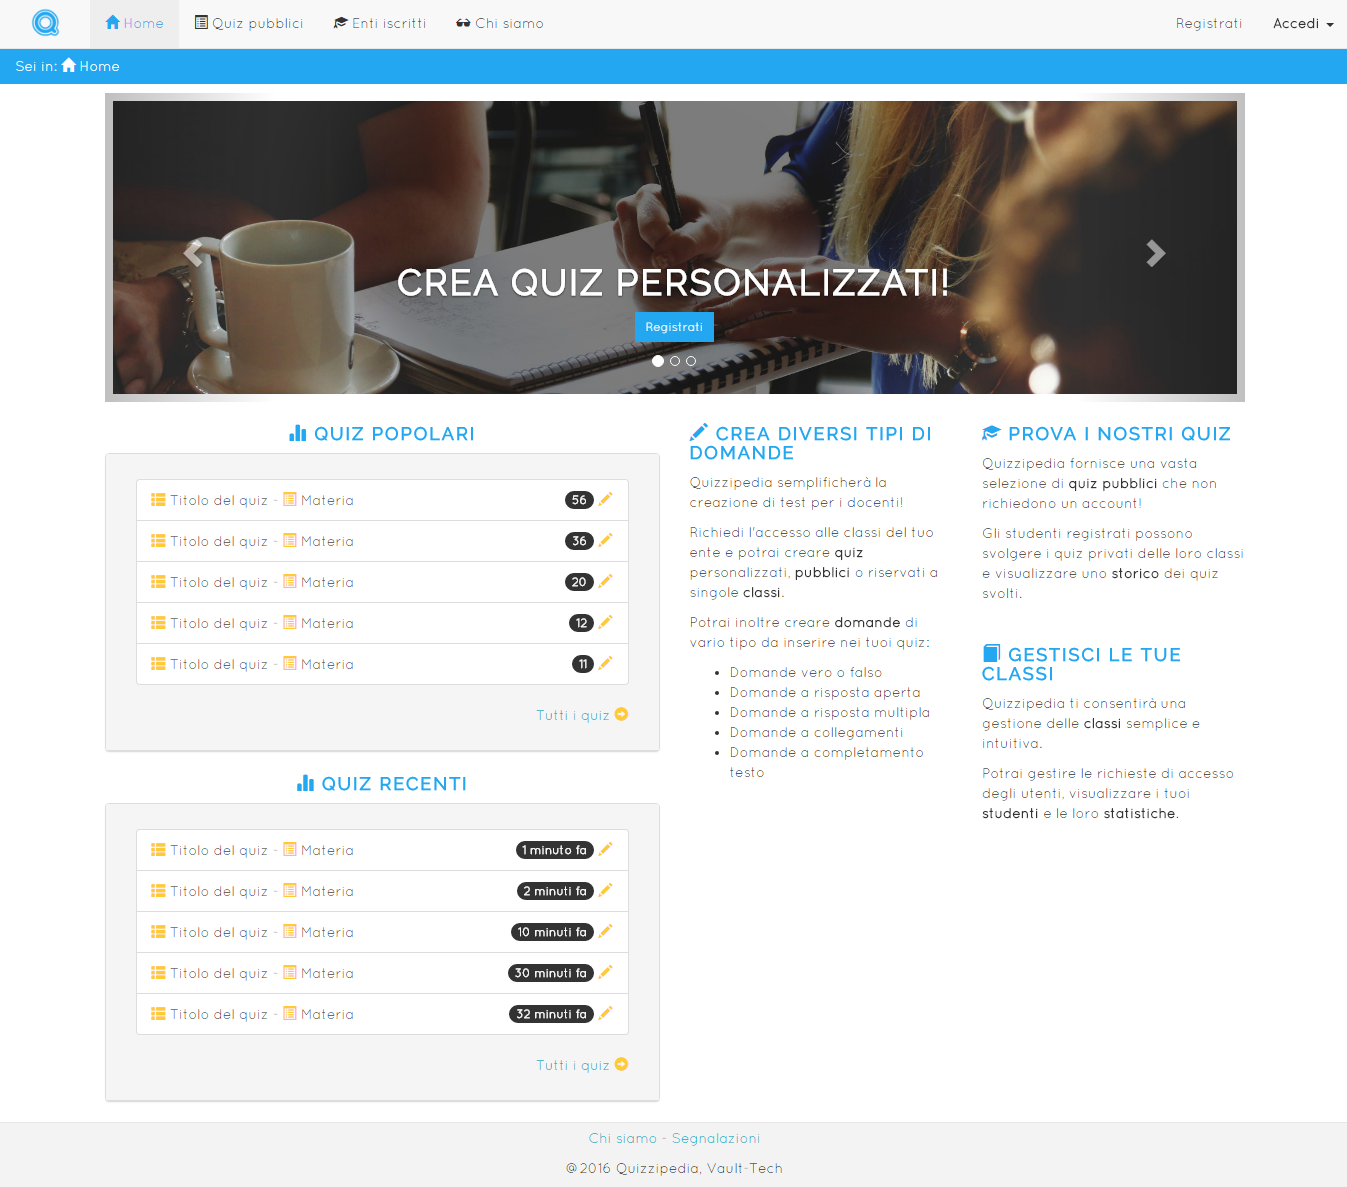
\includegraphics[scale=0.33]{Img/screen_HomepageGenerica.png}
		\caption{Schermata di homepage}
	\end{figure}
	Al primo accesso è consentito all'utente di autenticarsi, qualora già in possesso di un account valido, oppure registrarsi al sistema. Una volta autenticato la homepage varierà in base al tipo di account in uso (si vedano le sezioni successive per i vari tipi). 
	Anche senza autenticarsi sarà possibile usufruire dei servizi pubblici offerti da Quizzipedia, ma non vi sarà un salvataggio dei dati e delle statistiche. Si veda la \hyperref[pub]{sezione 4} per i vari servizi pubblici.
	
	\newpage
	\subsection{Registrazione}
	\begin{figure}[!h]
		\centering
		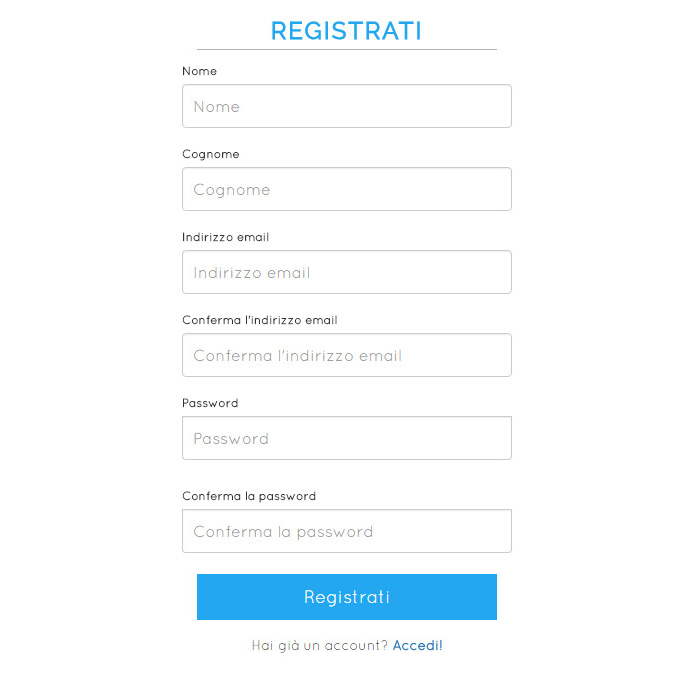
\includegraphics[scale=0.5]{Img/screen_Registrazione.png}
		\caption{Schermata di registrazione}
	\end{figure}
	Selezionare la voce 'Registrati' in alto a destra nella barra di navigazione porta alla pagina di registrazione.
	Per completare la registrazione è necessario inserire nell'apposito form:
	\begin{itemize}
		\item nome,
		\item cognome,
		\item indirizzo email valido,
		\item conferma dell'indirizzo email,
		\item password,
		\item conferma della password.
	\end{itemize}
	Se i dati sono stati inseriti correttamente, una volta effettuata la conferma cliccando sul pulsante 'Conferma', la registrazione sarà completata con successo.
	ATTENZIONE: l'uso di indirizzo email senza possibilità di accesso permetterà comunque la registrazione al sistema, ma comprometterà la funzione di recupero password.
	Verrà visualizzato un messaggio di errore nel caso le seguenti condizioni non siano verificate:
	\begin{itemize}
		\item l'indirizzo email immesso non deve essere associato a un account già esistente;
		\item l'indirizzo email deve avere un formato valido;
		\item la password immessa deve essere valida: compresa fra i 8 e i 16 caratteri;
		\item la password immessa e la sua conferma devono coincidere;
		\item tutti i campi devono essere riempiti.
	\end{itemize}
	
	
	\subsection{Autenticazione}
	\begin{figure}[!h]
		\centering
		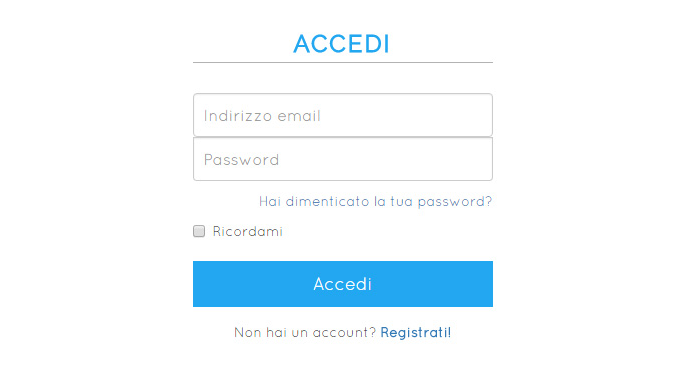
\includegraphics[scale=0.5]{Img/screen_Login.png}
		\caption{Schermata di autenticazione}
	\end{figure}
	Selezionare la voce 'Accedi' in alto a destra nella barra di navigazione per effettuare l'accesso al sistema. Per autenticarsi sarà necessario immettere il proprio indirizzo email e la password corrispondente. Se l'indirizzo email corrisponde a un account registrato e la password inserita è corretta l'autenticazione sarà completata con successo, altrimenti verrà visualizzato un messaggio di errore.
	
	\newpage
	\hypertarget{anc1}{ }
	\subsection{Recupero password}
	\begin{figure}[!h]
		\centering
		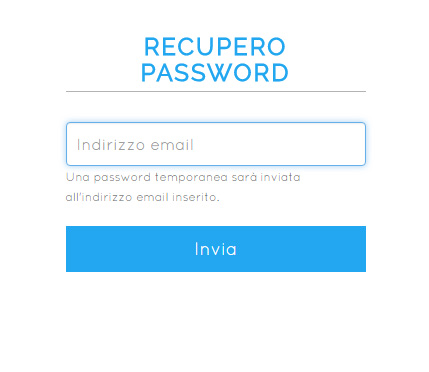
\includegraphics[scale=0.5]{Img/screen_RecuperoPwd.png}
		\caption{Schermata di recupero password}
	\end{figure}
	Nel caso l'utente non ricordi la propria password, è possibile ottenerne una temporanea compilando l'apposito form. Una volta inserito l'indirizzo email del suo account e confermata la richiesta, l'utente riceverà nella casella di posta una password temporanea che potrà utilizzare nel prossimo accesso. In caso di inserimento di email non presente nel sistema verrà visualizzato un messaggio di errore. È suggerito modificare la propria password dopo aver effettuato il recupero.
	
%	\subsection{Ricerca enti e classi}
%	NON DOVREBBE STARE QUI
%	\hyperlink{anc1}{clic}
	
	\newpage
	\section{Funzionalità pubbliche}
	\label{pub}
		A seguire vengono illustrate le funzionalità specifiche del prodotto che possono essere eseguite pubblicamente.
		
	\subsection{Ricerca quiz}
	\begin{figure}[!h]
		\centering
		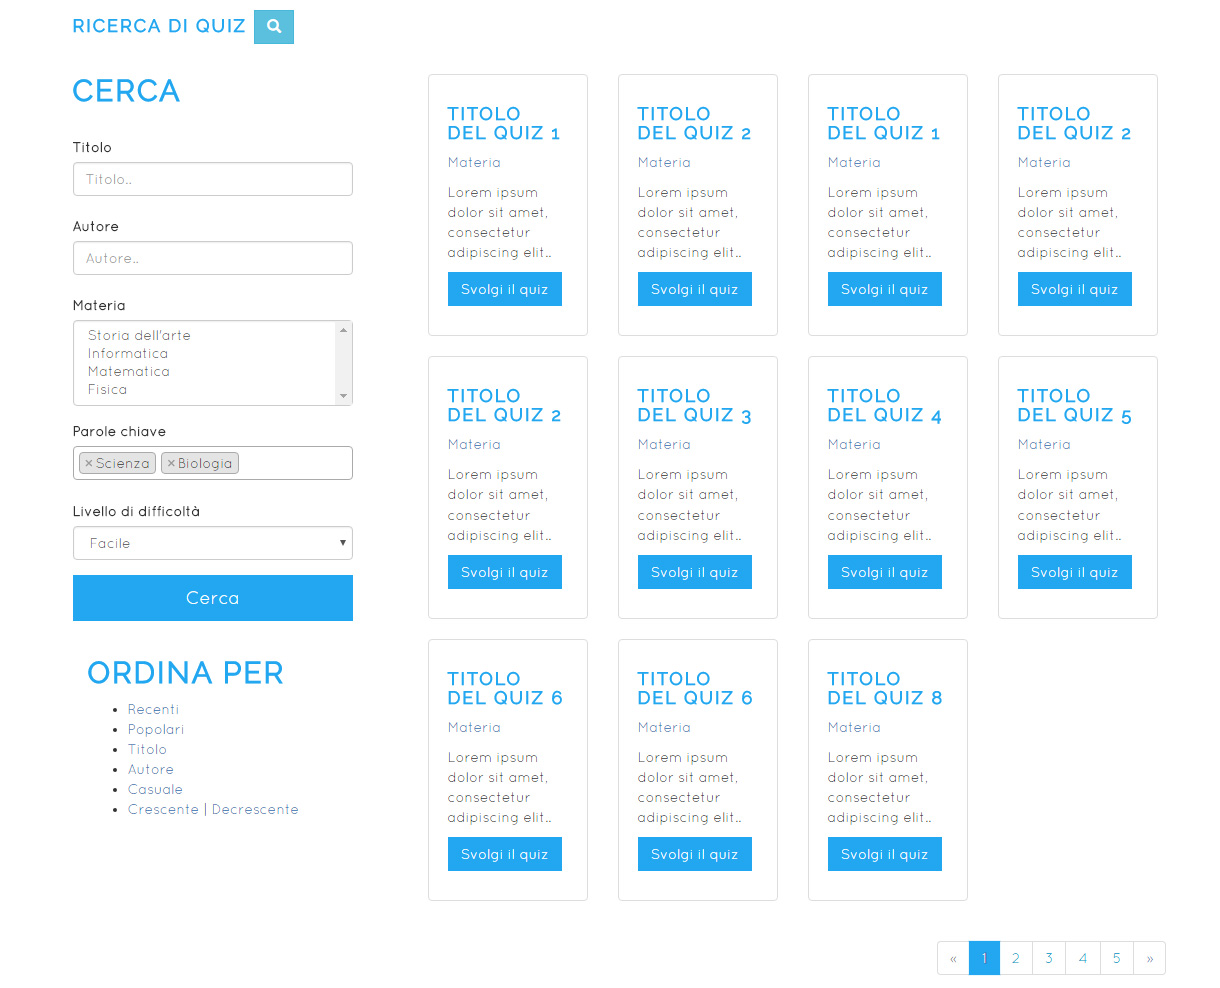
\includegraphics[scale=0.33]{Img/screen_RicercaQuiz.png}
		\caption{Schermata di ricerca quiz}
	\end{figure}
	 È possibile effettuare ricerche di quiz selezionando l'opzione 'Ricerca' nella barra di navigazione. La ricerca è personalizzabile attraverso diversi parametri:
	 \begin{itemize}
	 	\item titolo,
	 	\item autore,
	 	\item materia,
	 	\item parole chiave,
	 	\item livello di difficoltà.
	 \end{itemize}
	 Si noti che il creatore del quiz dovrà aver selezionato la visibilità del quiz 'pubblico' per poter essere trovato in questa ricerca. Sarà inoltre possibile ordinare i risultati secondo vari criteri, presenti sotto al tasto di conferma ricerca.
	 
	 \newpage
	 \subsection{Svolgimento quiz}
	 \begin{figure}[!h]
	 	\centering
	 	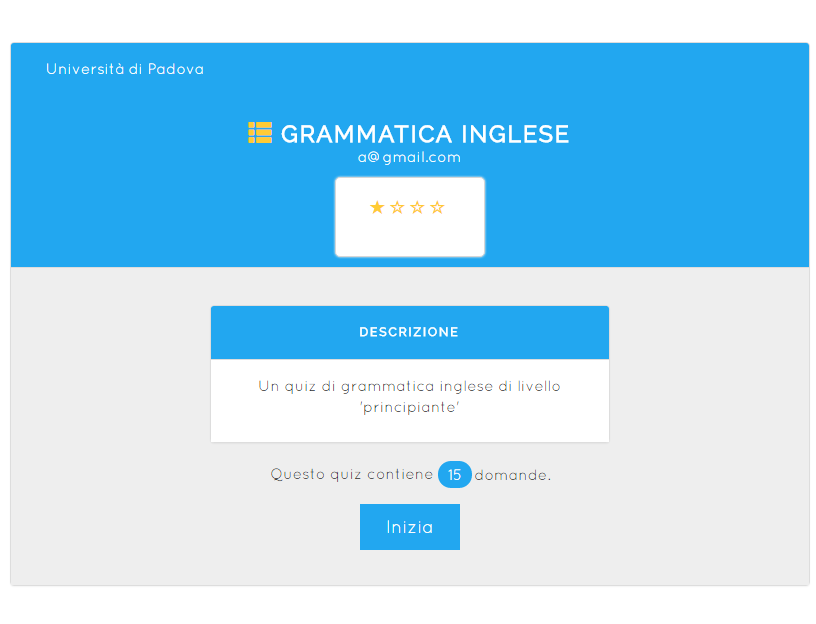
\includegraphics[scale=0.33]{Img/screen_SvolgimentoQuiz1.png}
	 	\caption{Schermata iniziale di svolgimento quiz}
	 \end{figure}
	 \begin{figure}[!h]
	 	\centering
	 	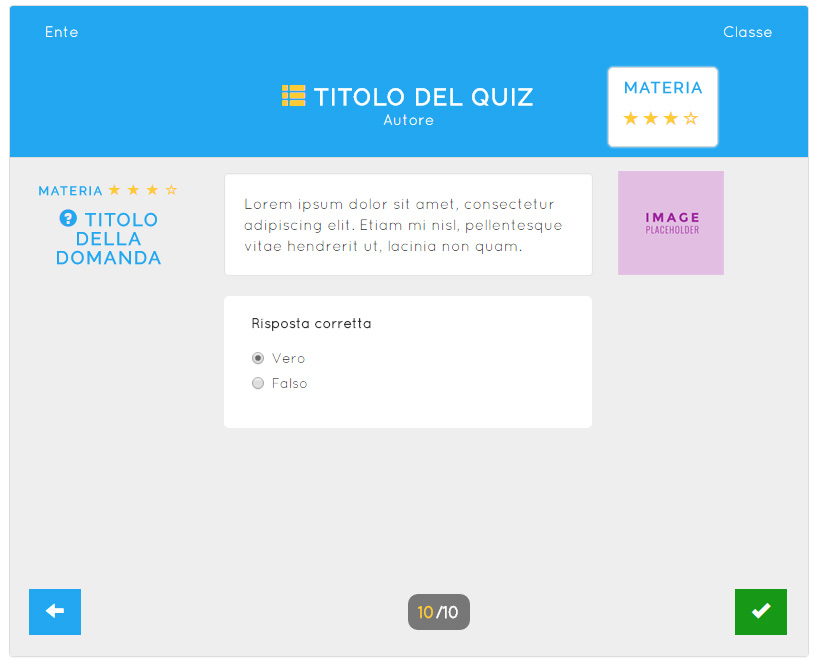
\includegraphics[scale=0.33]{Img/screen_SvolgimentoQuiz3.png}
	 	\caption{Schermata finale di svolgimento quiz}
	 \end{figure}
	 Una volta scelto il quiz e premuto sul tasto 'inizia' partirà l'esecuzione del quiz. Durante l'esecuzione e fino alla fine del quiz, l'utente potrà solo fare la sua scelta nelle varie domande, muoversi tra queste o decidere di annullare il quiz. Il sistema attualmente offre diversi tipi di domande, si veda l'\hyperref[domande]{appendice A} per la lista completa.
	 
	 \newpage
	 \begin{figure}[!h]
	 	\centering
	 	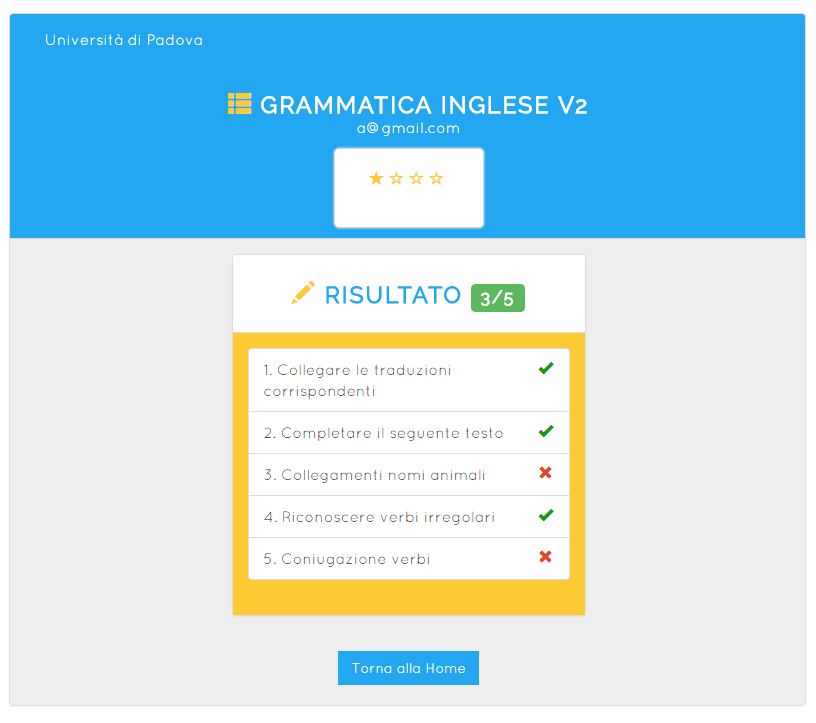
\includegraphics[scale=0.33]{Img/screen_EsitoQuiz.png}
	 	\caption{Schermata dell'esito quiz}
	 \end{figure}
	 Terminato il quiz verrà visualizzato il risultato come
	 \centra{numero di domande giuste / numero di domande totali} e si potrà uscire dall'ambiente di esecuzione del quiz.
	 
	 \newpage
	 \section{Utente autenticato}
	 Per utenti registrati nel sistema ma non all'interno di un istituzione sarà possibile godere delle funzionalità pubbliche, in aggiunta ad esse i risultati e le statistiche ora verranno salvati e saranno visualizzabili. Inoltre si avrà accesso alle funzioni base di gestione profilo, di ricerca di enti e classi e richieste di ruolo.

	 \subsection{Visualizzazione profilo}
	 \begin{figure}[!h]
	 	\centering
	 	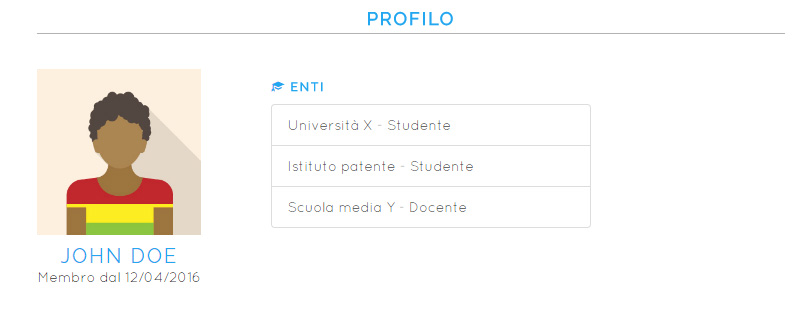
\includegraphics[scale=0.33]{Img/screen_ProfiloUtente.png}
	 	\caption{Schermata di visualizzazione profilo}
	 \end{figure}
	 Selezionando 'profilo' è possibile accedere alla pagina che mostra le informazioni di base dell'utente, come nome, cognome, le varie appartenenze agli enti e i ruoli dell'utente in essi.
	
	\subsection{Cambio password}
	
	\begin{figure}[!h]
		\centering
		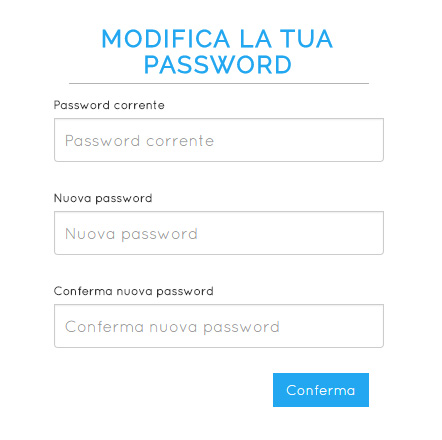
\includegraphics[scale=0.33]{Img/screen_CambioPassword.png}
		\caption{Schermata di cambio password}
	\end{figure}
	Il cambio password richiede di inserire la password attuale, una nuova password e la conferma di quest'ultima. Il numero di caratteri dovrà sempre essere compreso tra 8-16. È fortemente consigliato cambiare password dopo averla recuperata tramite email.
	
	\newpage
	\subsection{Richiesta ruoli e classi}
	\begin{figure}[!h]
		\centering
		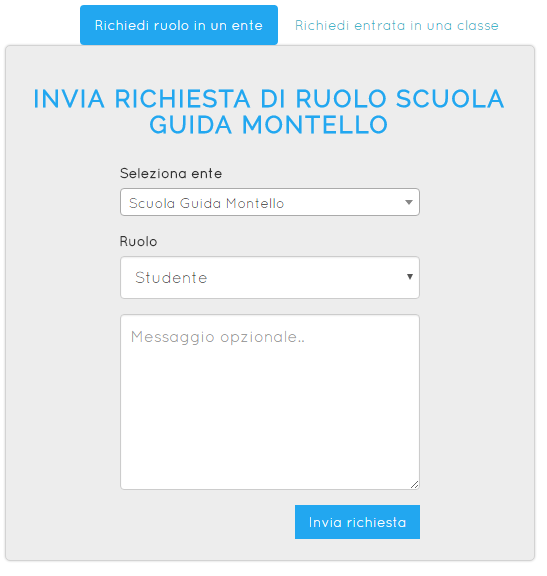
\includegraphics[scale=0.33]{Img/screen_RichiestaRuolo.png}
		\caption{Schermata di richiesta inserimento in un ente}
	\end{figure}	
	\begin{figure}[!h]
		\centering
		
\includegraphics[scale=0.33]{Img/screen_RichiestaClasse.png}
		\caption{Schermata di richiesta inserimento in una classe}
	\end{figure}
	Per essere inseriti in un istituto bisogna fare richiesta formale tramite il primo form, il menù a tendina fornisce la lista di istituti registrati nel sistema e il ruolo che in esso si desidera. È possibile fare richiesta di entrare in una classe dell'ente selezionato tramite il secondo form. Tali richieste rimangono pendenti fino alla loro approvazione o rifiuto da parte del responsabile.
	
	\newpage
	\subsection{Selezione ente}
	\begin{figure}[!h]
		\centering
		
\includegraphics[scale=0.33]{Img/screen_SelezioneEnte.png}
		\caption{Schermata di selezione ente}
	\end{figure}
	Appena autenticati se si è inseriti in un ente bisogna selezionare quest'ultimo dal menù di selezione ente.
	Se non viene selezionato alcun ente l'utente viene riconosciuto dal sistema come utente autenticato semplice, invece una volta selezionato si hanno accesso alle funzioni relative al tipo di account posseduto nell'ente scelto.
	 
	 \subsection{Visualizzazione storico dei quiz}
	 \begin{figure}[!h]
	 	\centering
	 	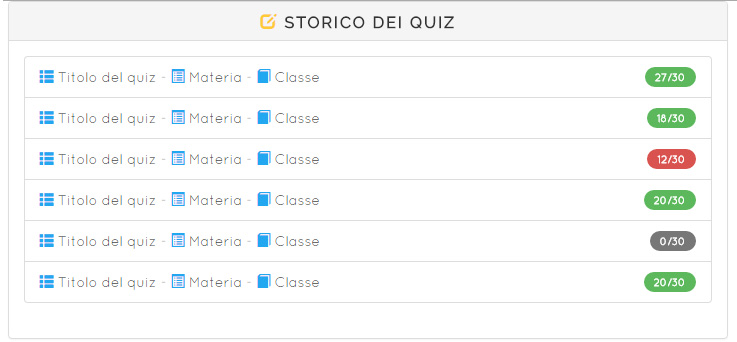
\includegraphics[scale=0.33]{Img/screen_StoricoQuiz.png}
	 	\caption{Schermata di visualizzazione storico dei quiz}
	 \end{figure}
	 È possibile visualizzare il proprio storico di quiz svolti, dove vengono riportati i risultati, le materie dei quiz, la classe se presente e il titolo. Risultato in verde si riferisce ad un quiz superato con successo, in rosso quelli non superati e in grigio i quiz privati pianificati ma non ancora svolti.
	  
	 \newpage
	 \section{Studente}
	 Dopo l'autenticazione, se si è stati accettati in un ente come studenti, sarà ora possibile svolgere i quiz privati assegnati, oltre naturalmente a ciò che era possibile svolgere da utente autenticato.
	 
	 \subsection{Homepage}
	 \begin{figure}[!h]
	 	\centering
	 	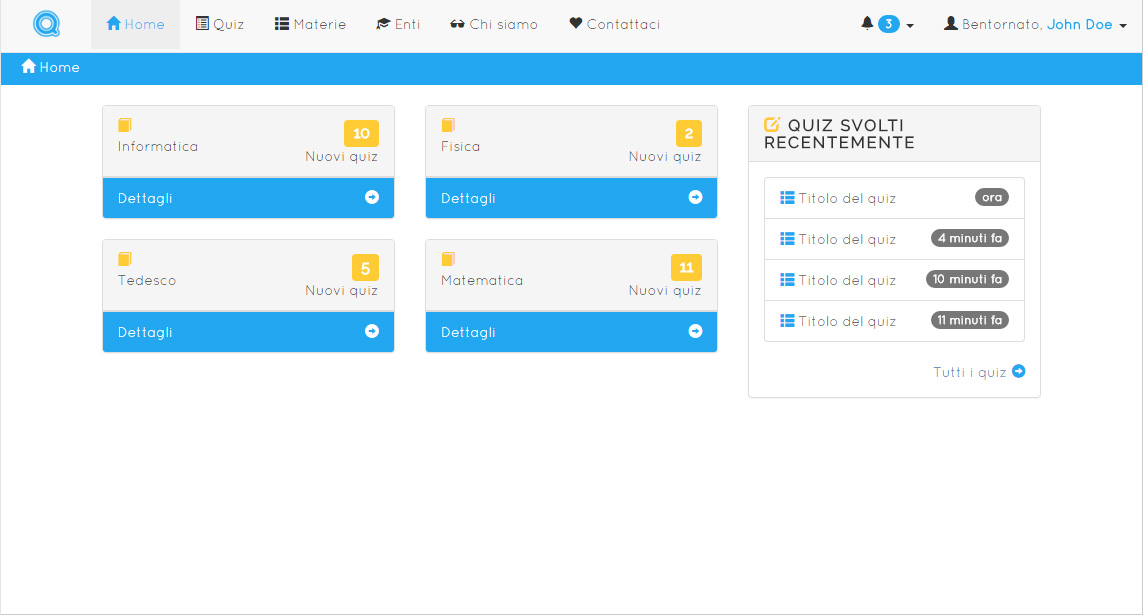
\includegraphics[scale=0.33]{Img/screen_HomepageStudente.png}
	 	\caption{Schermata di homepage studente}
	 \end{figure}
	 La homepage studente presenta subito i quiz privati più recenti disponibili per lo studente, divisi per classe di appartenenza, e una lista di quiz svolti di recente.
	 
	 \newpage
	 \subsection{Ricerca quiz privati}
	 \begin{figure}[!h]
	 	\centering
	 	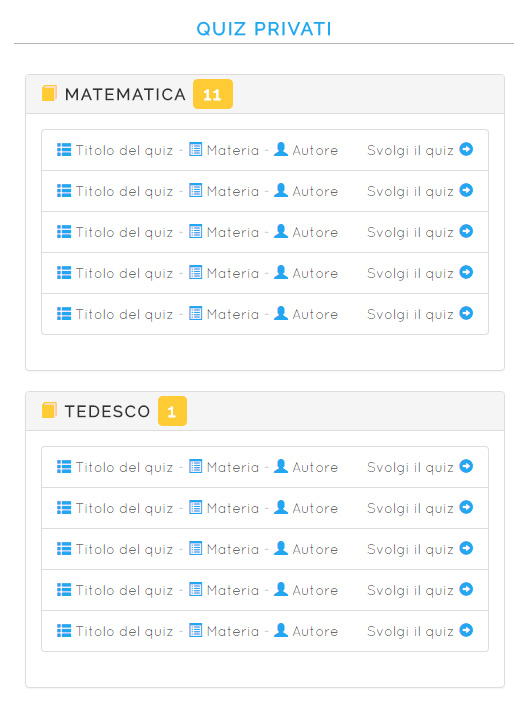
\includegraphics[scale=0.33]{Img/screen_ListaQuizPrivati.png}
	 	\caption{Schermata di quiz privati}
	 \end{figure}
	 Questa pagina elenca tutti i vari quiz privati pianificati per lo studente ma non ancora svolti, divisi per classe.
	 
	 
	 \newpage
	 \section{Docente}
	 Qualora l'utente sia in possesso di un account con permessi da docente, egli ha a disposizione una serie di funzionalità specifiche, come la gestione delle proprie classi e la visualizzazione delle relative statistiche, la possibilità di creare domande e quiz e gestirli.
	 
	 \subsection{Homepage}
	 \begin{figure}[!h]
	 	\centering
	 	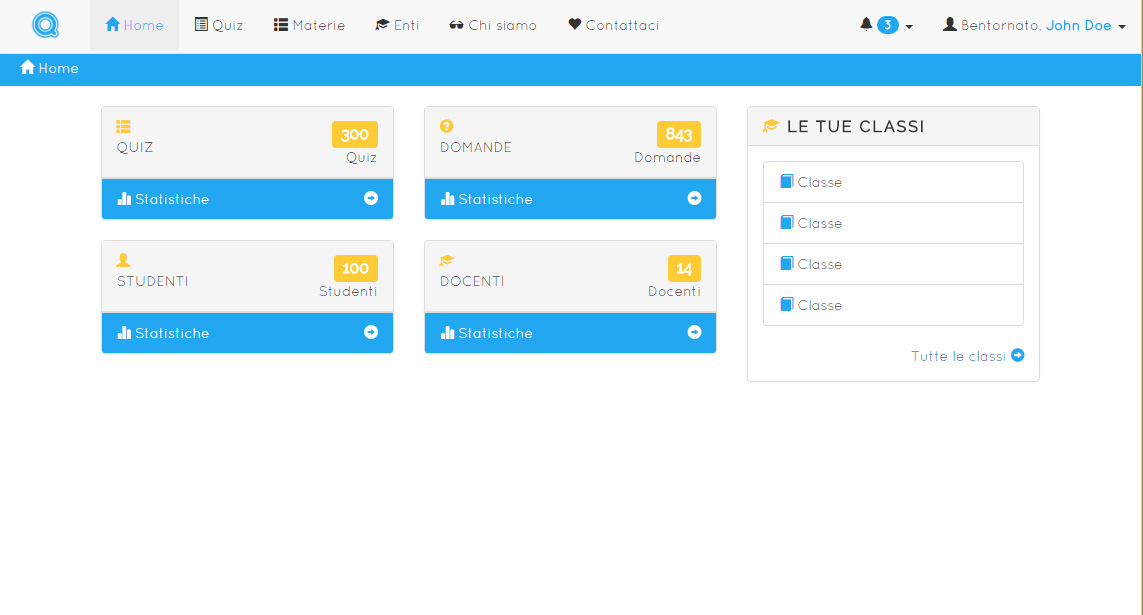
\includegraphics[scale=0.33]{Img/screen_HomepageDocente.png}
	 	\caption{Schermata di homepage docente}
	 \end{figure}
	 Nella homepage del docente saranno visualizzate le classi in cui il docente insegna e le statistiche relative a domande, quiz, studenti e docenti dell'ente in cui ha effettuato l'accesso.
	 
%	 \subsection{Gestione classe}
	 
	 \subsection{Gestione quiz}
	 \begin{figure}[!h]
	 	\centering
	 	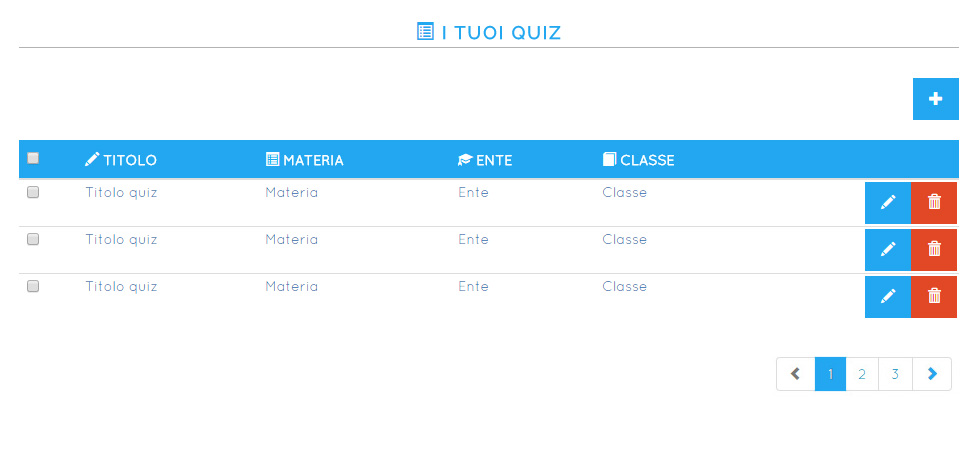
\includegraphics[scale=0.33]{Img/screen_GestioneQuiz.png}
	 	\caption{Schermata di gestione quiz}
	 \end{figure}
	 Qui vengono elencati tutti i propri quiz personali creati ed è possibile iniziare la creazione di un nuovo quiz o eliminare uno già esistente.
	 
	 \newpage
	 \subsection{Creazione quiz}
	 \begin{figure}[!h]
	 	\centering
	 	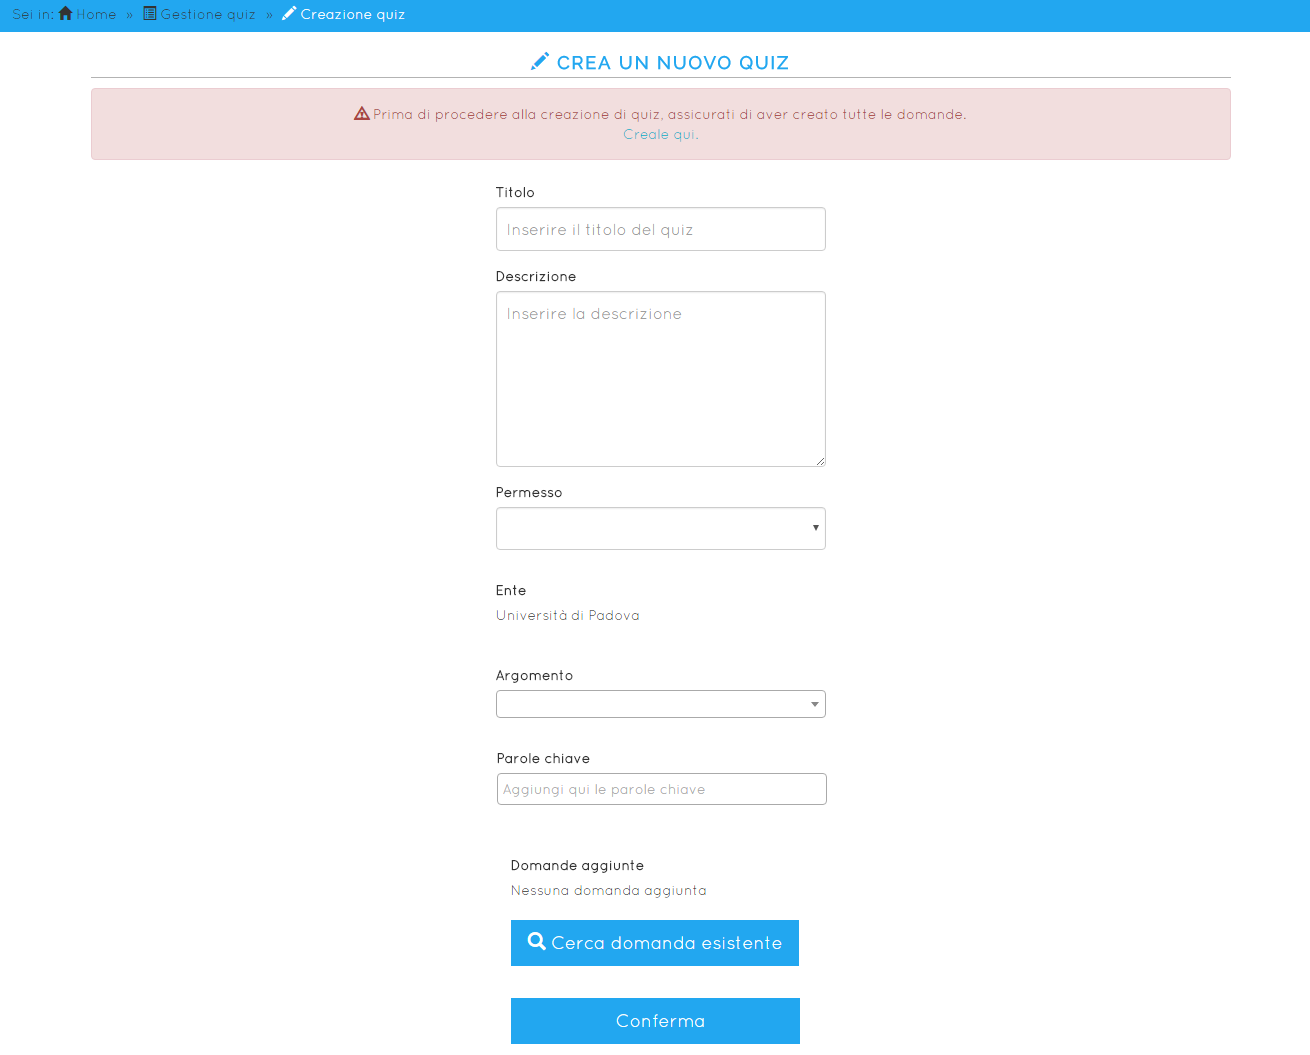
\includegraphics[scale=0.33]{Img/screen_CreazioneQuiz.png}
	 	\caption{Schermata di creazione quiz}
	 \end{figure}
	 Il wizard di creazione dei quiz permette di inserire:
	 \begin{itemize}
	 	\item il titolo,
	 	\item una breve descrizione del quiz,
	 	\item un immagine allegata,
	 	\item la materia,
	 	\item il livello di difficoltà,
	 	\item le varie parole chiave associate,
	 	\item il tipo di permesso (visibilità pubblica o privata),
	 	\item l'ente di appartenenza (di default il proprio),
	 	\item la classe a cui è destinato il quiz (qualora sia selezionato permesso privato),
	 	\item le varie domande che verranno associate al quiz.
	 \end{itemize}
	 Per aggiungere le domande si aprirà un menù che permetterà di cercare nel \gl{database} delle domande (pubbliche o quelle personali già create) oppure crearne al momento. Per dettagli sulla creazione domande si rimanda all'\hyperref[domande]{appendice A}.
	 
	 \newpage
	 \subsection{Gestione domande}
	 \begin{figure}[!h]
	 	\centering
	 	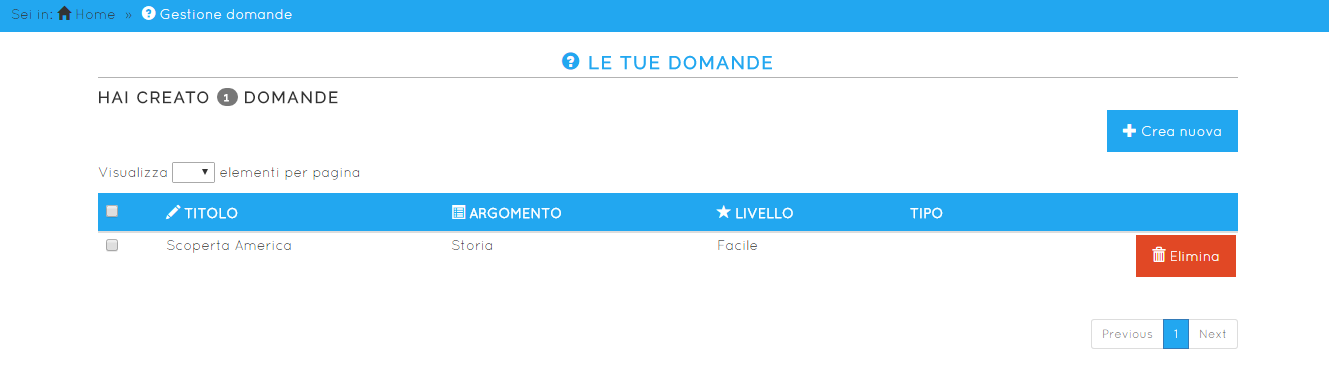
\includegraphics[scale=0.33]{Img/screen_gestioneDomande.png}
	 	\caption{Schermata di gestione domande}
	 \end{figure}
	 Qui vengono elencate tutte le proprie domande personali già create ed è possibile iniziare la creazione di una nuova domanda o eliminare una già esistente. Per dettagli sulla creazione domande si rimanda all'\hyperref[domande]{appendice A}.
	 
	 \subsection{Visualizzazione statistiche}
	 \begin{figure}[!h]
	 	\centering
	 	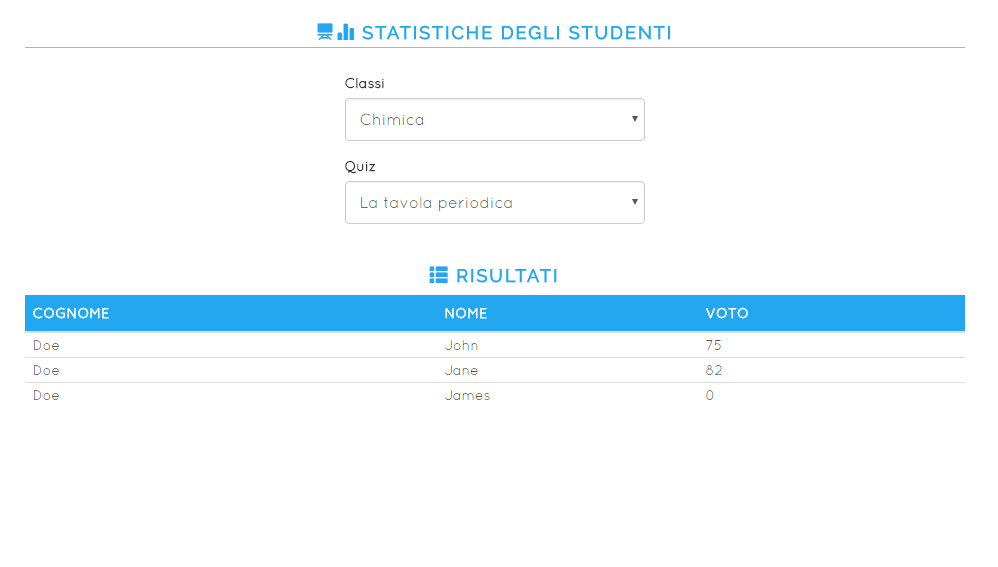
\includegraphics[scale=0.33]{Img/screen_StatisticheStudenti.png}
	 	\caption{Schermata di visualizzazione statistiche degli studenti}
	 \end{figure}
	 Qui è possibile visualizzare per i propri studenti i risultati dei quiz sottoposti, applicando opzionalmente dei filtri specifici, come la classe di appartenenza o il titolo del quiz.
	 
	 \newpage
	 \section{Responsabile}
	 Qualora si sia in possesso di un account di tipo 'responsabile' si hanno a disposizione un set di funzionalità uniche per la gestione del proprio ente, come gli utenti che ne fanno parte, le relative classi e gli argomenti.
	 
	 \subsection{Homepage}
	 \begin{figure}[!h]
	 	\centering
	 	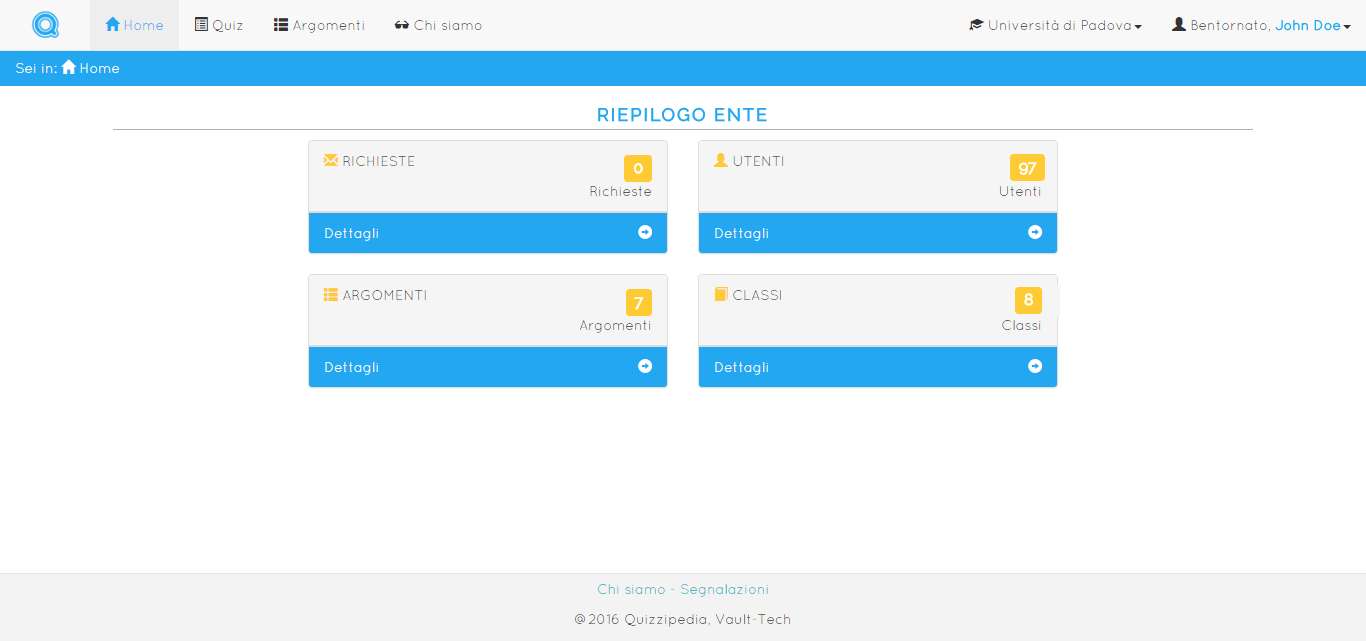
\includegraphics[scale=0.33]{Img/screen_HomepageResponsabile.png}
	 	\caption{Schermata di homepage responsabile}
	 \end{figure}
	 Nella homepage del responsabile verranno visualizzate le varie richieste indirizzate all'ente.
	 
	 \subsection{Gestione argomento}
	 \begin{figure}[!h]
	 	\centering
	 	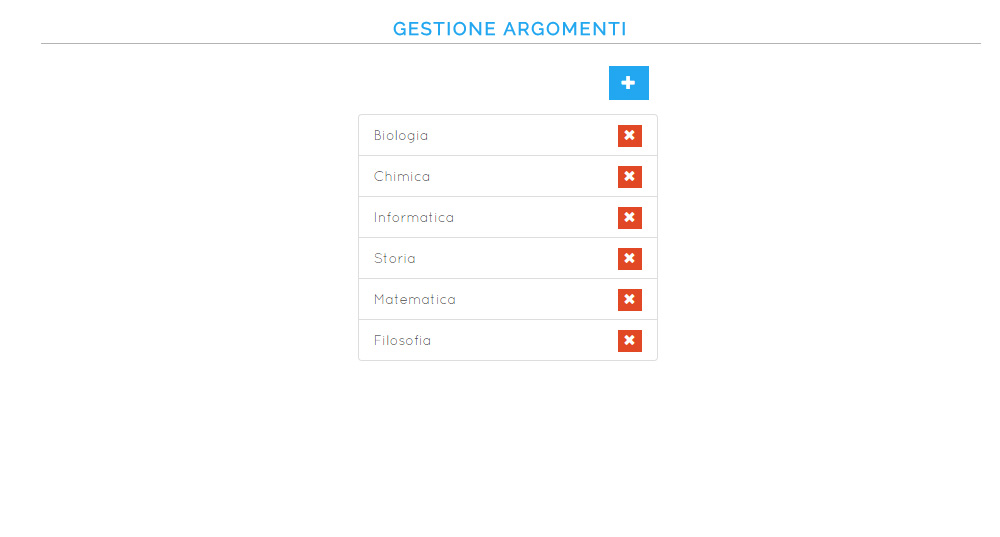
\includegraphics[scale=0.33]{Img/screen_GestioneArgomenti.png}
	 	\caption{Schermata di gestione argomenti}
	 \end{figure}
	 I vari argomenti vengono utilizzati dal sistema per classificare quiz e domande per ogni ente. Ogni responsabile può definire la propria lista argomenti per organizzare meglio il proprio materiale: è possibile aggiungere o eliminare argomenti dalla lista tramite il form sopra illustrato.
	 
	 \subsection{Gestione utenti}
	 \begin{figure}[!h]
	 	\centering
	 	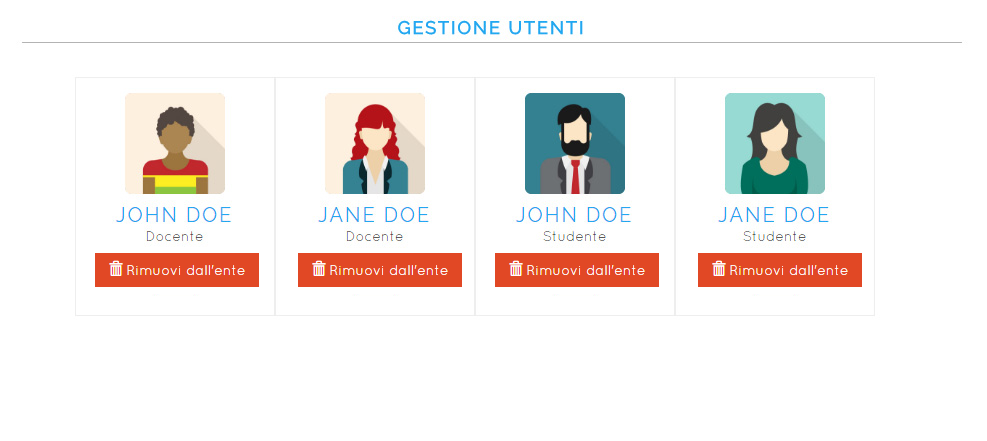
\includegraphics[scale=0.33]{Img/screen_GestioneUtenti.png}
	 	\caption{Schermata di gestione utenti}
	 \end{figure}
	 Dalla schermata di gestione utenti il responsabile può visualizzare tutti gli utenti che hanno un ruolo nel proprio ente, e rimuoverli se desiderato.
	 
	 \subsection{Gestione ente e classi}
	 \begin{figure}[!h]
	 	\centering
	 	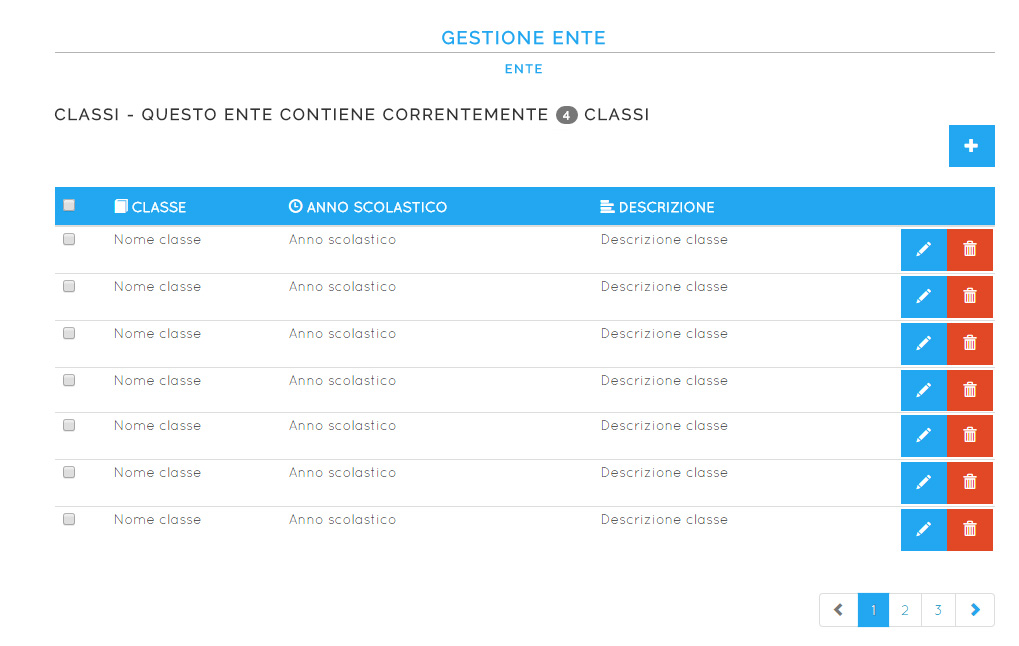
\includegraphics[scale=0.33]{Img/screen_GestioneEnteClassi.png}
	 	\caption{Schermata di gestione classi}
	 \end{figure}

	 Nella gestione classi è possibile modificare, eliminare o aggiungere classi dal proprio istituto. Per ogni classe si possono inserire o rimuovere studenti e docenti.
	 
	 \newpage
	 \subsection{Gestione richieste}
	 \begin{figure}[!h]
	 	\centering
	 	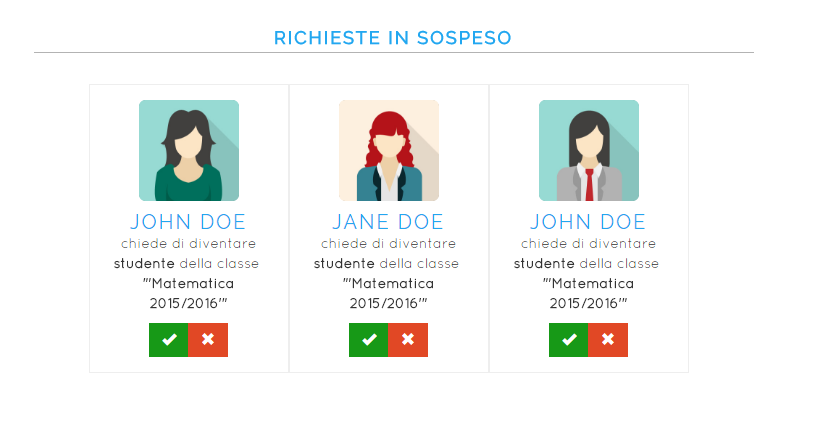
\includegraphics[scale=0.33]{Img/screen_GestioneRichieste.png}
	 	\caption{Schermata di gestione richieste}
	 \end{figure}
	 Dalla schermata di gestione utenti il responsabile può visualizzare le richieste in sospeso effettuate dagli altri utenti e accettarle o rifiutarle.
	 
	 \newpage
	 \section{Segnalazione problemi e richieste}
	 \begin{figure}[!h]
	 	\centering
	 	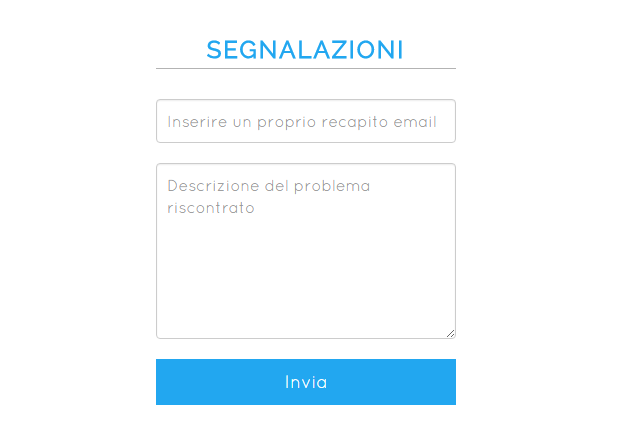
\includegraphics[scale=0.33]{Img/screen_Segnalazioni.png}
	 	\caption{Schermata di segnalazione problemi e richieste}
	 \end{figure}
	 Dalla schermata di segnalazione problemi e richieste un utente di qualsiasi tipo può segnalare anomalie riscontrate durante l'utilizzo del prodotto all'amministratore di sistema, può anche fare una richiesta formale per l'inserimento di un proprio ente all'interno del prodotto e esserne nominato responsabile.
	 
	 \newpage
	 \appendix
	 
	 \section{Tipi di domande}
	 \label{domande}
	 A seguire sono elencati vari tipi di domande utilizzabili nel sistema.
	 
	 \subsection{Vero o falso}
	 \begin{figure}[!h]
 	 	\centering
 	 	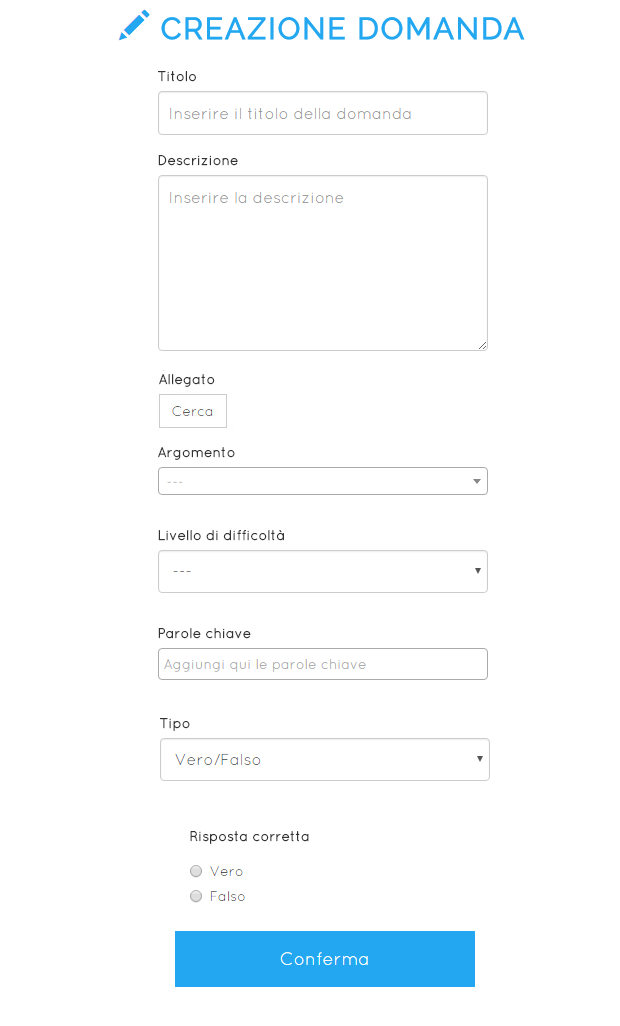
\includegraphics[scale=0.33]{Img/screen_CreazioneDomandaVF.png}
 	 	\caption{Schermata di creazione domanda vero o falso}
	 \end{figure}
	 Le domande di tipo 'vero o falso' consentono di interrogare gli studenti sulla veridicità di un'affermazione. 
	 Per creare una domanda vero o falso è necessario compilare nel relativo form:
	 \begin{itemize}
 	 	\item titolo della domanda,
 	 	\item descrizione della domanda,
 	 	\item allegato multimediale (immagine, audio o video) opzionale,
 	 	\item materia,
 	 	\item livello di difficoltà,
 	 	\item parole chiave che identificano la domanda.
	 \end{itemize}
	 È infine necessario indicare la risposta corretta, scegliendo 'vero' o 'falso' nell'apposita checkbox.

	 
	 \newpage
	 \subsection{Risposta multipla}
	 \begin{figure}[!h]
	 	\centering
	 	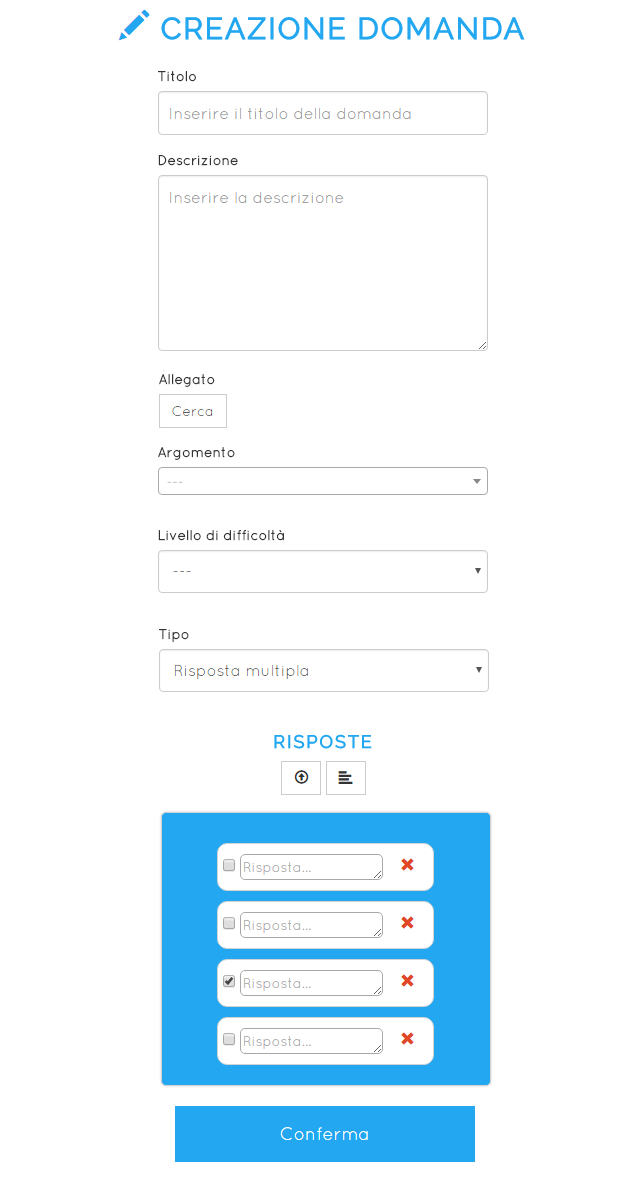
\includegraphics[scale=0.33]{Img/screen_CreazioneDomandaRMultipla.png}
	 	\caption{Schermata di creazione domanda a risposta multipla}
	 \end{figure}
	 Le domande di tipo 'a risposta multipla' presentano quesiti con molteplici risposte possibili, di cui una o più sono corrette.
	 Per creare una domanda a risposta multipla è necessario compilare nel relativo form:
	 \begin{itemize}
	 	\item titolo della domanda,
	 	\item descrizione della domanda,
	 	\item allegato multimediale (immagine, audio o video) opzionale,
	 	\item materia,
	 	\item livello di difficoltà,
	 	\item parole chiave che identificano la domanda.
	 \end{itemize}
	 È poi necessario creare tutte le possibili risposte della domanda, sia corrette che errate. Cliccando nei rispettivi pulsanti è possibile creare una risposta di tipo multimediale o testuale. Nel caso venga creata una risposta multimediale sarà necessario effettuare l'upload del file immagine, audio o video desiderato, mentre nel caso venga creata una risposta testuale sarà necessario scrivere il testo della risposta nell'apposita casella di testo.
	 Infine dovranno essere indicate le risposte corrette spuntando le checkbox corrispondenti.
	 
	 \newpage
	 \subsection{A completamento}
	 \begin{figure}[!h]
	 	\centering
	 	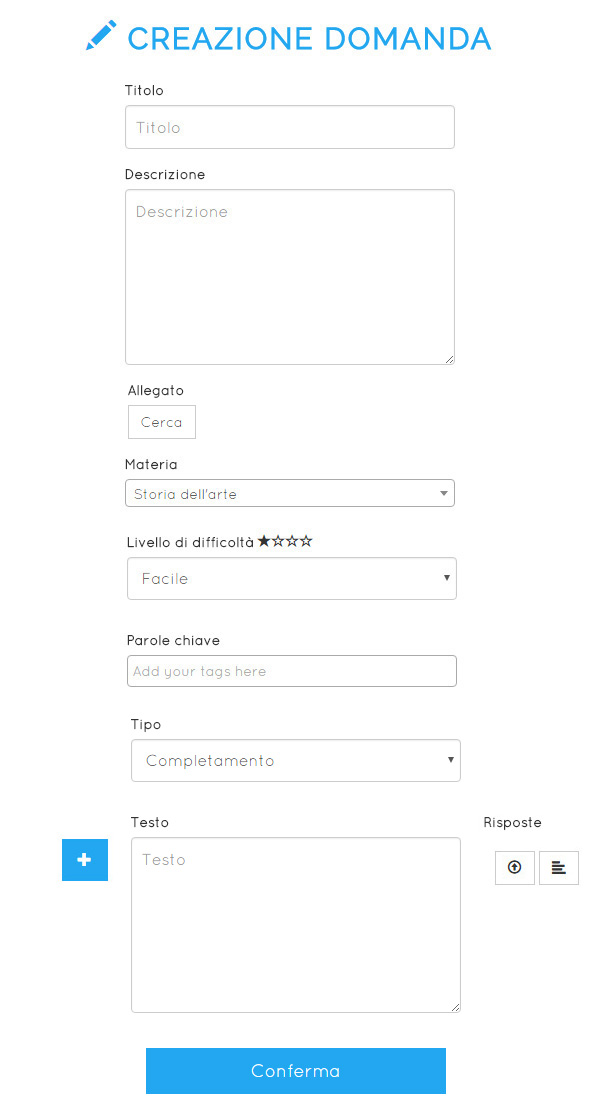
\includegraphics[scale=0.33]{Img/screen_CreazioneDomandaCompletamento.png}
	 	\caption{Schermata di creazione domanda a completamento testo}
	 \end{figure}
	 Le domande di tipo 'a completamento testo' presentano un testo con dei buchi dove devono essere inseriti i pezzi di testo o i file multimediali mancanti.
	 Per creare una domanda a completamento testo è necessario compilare nel relativo form:
	 \begin{itemize}
	 	\item titolo della domanda,
	 	\item descrizione della domanda,
	 	\item materia,
	 	\item livello di difficoltà,
	 	\item parole chiave che identificano la domanda,
	 	\item le parti di testo con i buchi da completare,
	 	\item le risposte relative ai buchi.
	 \end{itemize}
	 Il docente tramite il tasto aggiungi può aggiungere pezzi di testo, ad ogni aggiunta di pezzi di testo verrà inserito anche il buco dove andrà inserita una risposta (i buchi si riconosceranno da un numero ID crescente dispari tra i blocchi di testo). Infine le risposte dovranno essere aggiunte con il tasto apposito, associando la risposta alla posizione giusta corrispondente tramite il selettore di ID, è possibile inserire risposte con nessuna corrispondenza dandogli ID "-1". Si presti attenzione al fatto che ogni buco nel testo deve avere una risposta corrispondente.
	 
	 \newpage
	 \subsection{Risposta aperta}
	 \begin{figure}[!h]
	 	\centering
	 	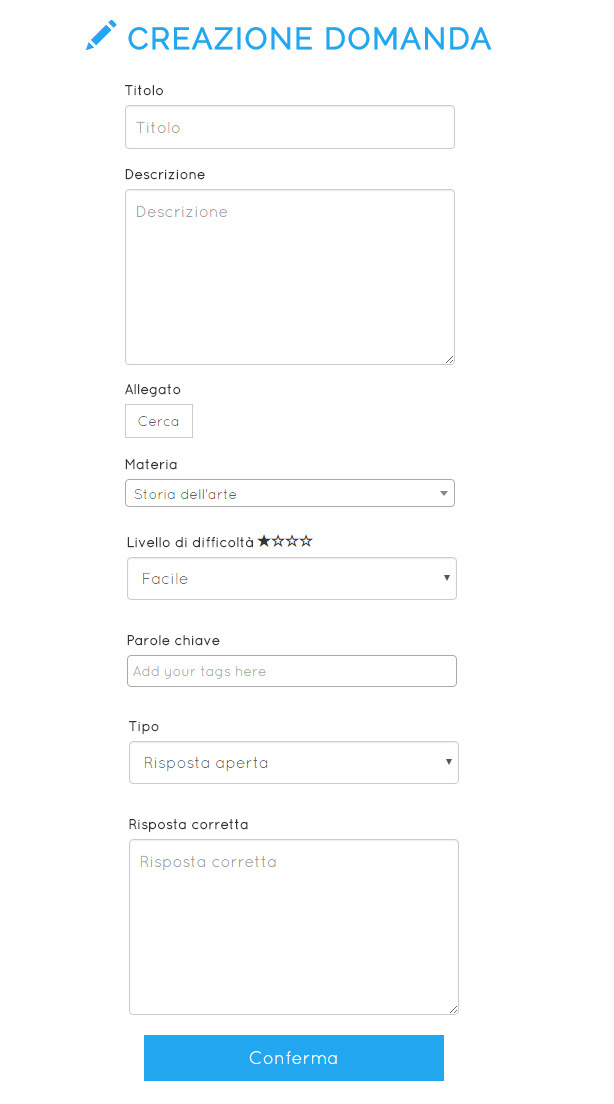
\includegraphics[scale=0.33]{Img/screen_CreazioneDomandaAperta.png}
	 	\caption{Schermata di creazione domanda a risposta aperta}
	 \end{figure}
	 Le domande di tipo 'a risposta aperta' presentano quesiti con una sola risposta testuale. È suggerito creare domande a risposta aperta soltanto per quesiti con risposte brevi e chiare, come date, nomi o parole singole. 
	 Per creare una domanda a risposta aperta è necessario compilare nel relativo form:
	 \begin{itemize}
	 	\item titolo della domanda,
	 	\item descrizione della domanda,
	 	\item allegato multimediale (immagine, audio o video) opzionale,
	 	\item materia,
	 	\item livello di difficoltà,
	 	\item parole chiave che identificano la domanda,
	 	\item testo della risposta corretta.
	 \end{itemize}
	 In esecuzione il controllo della risposta non sarà case sensitive (ovvero caratteri in maiuscolo verranno trattati come minuscolo).
	 
	 \newpage
	 \subsection{A collegamenti}
	 \begin{figure}[!h]
	 	\centering
	 	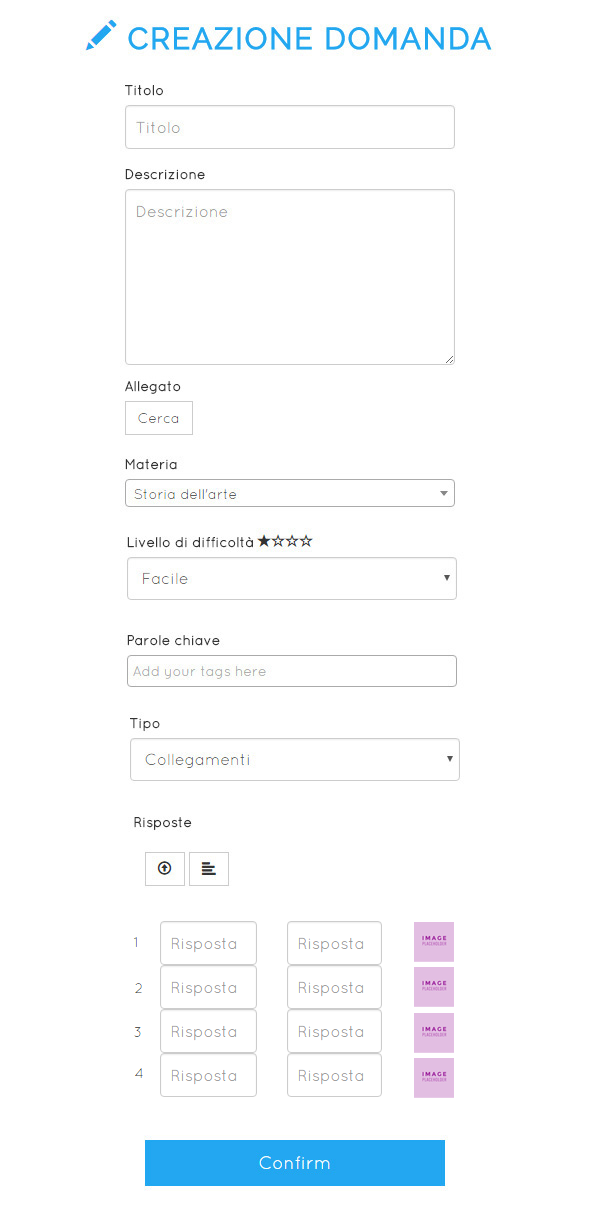
\includegraphics[scale=0.33]{Img/screen_CreazioneDomandaCollegamenti.png}
	 	\caption{Schermata di creazione domanda a collegamenti}
	 \end{figure}
	 Le domande di tipo 'a collegamenti' presentano porzioni di testo o file multimediali da collegare a coppie per formare una risposta corretta.
	 Per creare una domanda a collegamenti è necessario compilare nel relativo form:
	 \begin{itemize}
	 	\item titolo della domanda,
	 	\item descrizione della domanda,
	 	\item allegato multimediale (immagine, audio o video) opzionale,
	 	\item materia,
	 	\item livello di difficoltà,
	 	\item parole chiave che identificano la domanda,
	 	\item elementi della parte sinistra da collegare (testo o allegato),
	 	\item elementi della parte destra da collegare (testo o allegato).
	 \end{itemize}
	 Tramite il tasto aggiungi si possono inserire elementi nella relative parti di tipo testuale o allegato, per stabilire quali elementi sono accoppiati bisogna settare il loro ID in modo che corrisponda.
	 
	 \section{Glossario}
	 \label{gl} 
	 
	 \subsection{Browser}
	 Programma che consente di usufruire dei servizi di connettività in Internet, o di una rete di computer.
	 
	 \subsection{Cookies}
	 I cookie HTTP (più comunemente denominati cookie web, o per antonomasia cookie) sono un tipo
	 particolare di magic cookie, una sorta di gettone identificativo, usato dai server web per poter
	 riconoscere i browser durante comunicazioni con il protocollo HTTP usato per la navigazione web.
	 Tale riconoscimento permette di realizzare meccanismi di autenticazione, conservazione di dati utili
	 alla sessione di navigazione, di associare dati memorizzati dal server e di tracciare la navigazione dell’utente.
	 
	 \subsection{CSS3}
	 Il CSS (Cascading Style Sheets) è un linguaggio usato per definire la formattazione di documenti HTML, XHTML e XML. CSS3 è l’ultimo standard approvato al momento.

	 \subsection{Database}
	 È una base di dati, cioè un archivio o un insieme di archivi contenenti informazioni strutturate e
	 collegate tra loro secondo un particolare modello logico (relazionale, gerarchico, a oggetti, etc.),
	 offrendo una gestione efficiente dei dati che vi sono contenuti.

	 \subsection{Google Chrome}
	 Browser web sviluppato da Google.
	 
	 \subsection{HTML5}
	 L’HTML5 `e un linguaggio di markup per la strutturazione delle pagine web divenuto standard W3C nell’ottobre 2014.

	 \subsection{Internet Explorer}
	 Browser web sviluppato da Microsoft Windows. La nuova versione del browser è la Edge, a differenza delle precedenti che portavano il nome di Internet Explorer.

	 \subsection{JavaScript}
	 Linguaggio di programmazione interpretato, generalmente utilizzato nella gestione degli eventi.
	 Implementa un paradigma basato sia sugli oggetti che sulla programmazione funzionale.
	 
	 \subsection{Mozilla Firefox}
	 Browser web open source sviluppato da Mozilla Foundation. Risulta essere il terzo browser più diffuso.
	
	 \subsection{Safari}
 	 Safari è un browser web sviluppato da Apple Inc.
 	 
 	 \subsection{Software}
 	 Un software, in informatica, è l’informazione o le informazioni utilizzate da uno o più sistemi informatici
 	 e memorizzate su uno o più supporti informatici. Tali informazioni possono essere quindi rappresentate da uno o più programmi, oppure da uno o più dati, oppure da una combinazione
 	 delle due.
 	 
 	 \subsection{Web}
 	 Il Web, abbreviazione di World Wide Web, è uno dei principali servizi di Internet che permette di
 	 navigare e usufruire di un insieme vastissimo di contenuti (multimediali e non) collegati tra loro
 	 attraverso legami (link), e di ulteriori servizi accessibili a tutti o ad una parte selezionata degli
 	 utenti di Internet.
 	 
	
\end{document}
